\documentclass[11pt]{article}

%----------------------------------------------------------------
% 1. DOCUMENT SETUP & TYPOGRAPHY
%----------------------------------------------------------------
%\usepackage[TS1, T1]{fontenc}               % Font encoding for output
%\usepackage[adobe-utopia]{mathdesign}       % Adobe Utopia font
\usepackage{microtype}                      % Improves typography (line breaking, spacing)
\usepackage{setspace}                       % For line spacing control (e.g., \doublespacing)
\usepackage{soul}                           % For strikethrough and underlining (\ul)
\usepackage{dirtytalk}                      % For inline quotations
\usepackage{titling}                        % Control over \maketitle
\usepackage{epigraph}                       % For epigraphs

%----------------------------------------------------------------
% 2. PAGE LAYOUT & LINKS
%----------------------------------------------------------------
\usepackage{geometry}                       % For page margins and layout
\usepackage{pdflscape}                      % For landscape pages
\usepackage[dvipsnames]{xcolor}             % Color support
\usepackage[colorlinks=true]{hyperref}      % PDF hyperlinks (should be loaded late)

%----------------------------------------------------------------
% 3. MATHS & THEOREMS
%----------------------------------------------------------------
\usepackage[leqno]{amsmath}                        % Core maths tools

% Theorem-like environments
\newtheorem{theorem}{Theorem}[section]
\newtheorem{assumption}{Assumption}
\newtheorem{corollary}[theorem]{Corollary}
\newtheorem{proposition}{Proposition}[section]
\newtheorem{lemma}[theorem]{Lemma}
\newtheorem{conjecture}{Conjecture}[section]
\newenvironment{proof}[1][Proof]{\noindent\textbf{#1.} }{\ \rule{0.5em}{0.5em}}

% Custom math operators
\DeclareMathOperator{\E}{\mathbb{E}}
\DeclareMathOperator{\R}{\mathbb{R}}
\DeclareMathOperator{\plim}{\mbox{plim}}
\DeclareMathOperator{\todis}{\xrightarrow{d}}
\DeclareMathOperator{\normal}{\mathcal{N}}
\DeclareMathOperator{\var}{\mbox{var}}
\DeclareMathOperator{\prob}{\mathbb{P}}

%----------------------------------------------------------------
% 4. TABLES, FIGURES & GRAPHICS
%----------------------------------------------------------------
\usepackage{graphicx}                       % For including images
\usepackage{caption, subcaption}            % Enhanced captions for figures and tables
\usepackage{booktabs}                       % High-quality table rules (\toprule, \midrule, \bottomrule)
\usepackage{dcolumn}                        % Align table columns on a decimal point
\usepackage{longtable, threeparttable, threeparttablex} % For long tables and tables with notes
\usepackage{multirow, adjustbox}            % For multi-row cells and adjusting box content
\usepackage{rotating}                       % For rotating elements (e.g., sidewaystable)
\usepackage{tikz}                           % For drawing graphics
\usetikzlibrary{positioning}

%----------------------------------------------------------------
% 5. LISTS
%----------------------------------------------------------------
\usepackage{enumitem}                       % Advanced control over lists

%----------------------------------------------------------------
% 6. BIBLIOGRAPHY (Author-Year Style)
%----------------------------------------------------------------
\usepackage[
    backend=biber,      % Use the Biber engine
    style=authoryear,   % Set main style to author-year
    citestyle=authoryear-comp, % Compress citations (e.g., Author 2020, 2021)
    natbib=true,        % Allow use of natbib commands like \citet and \citep
    maxcitenames=2,     % Max authors to show in citation before "et al."
    maxbibnames=99,     % Max authors to show in the bibliography
    uniquelist=false    % Prevents adding initials to distinguish authors
]{biblatex}
\addbibresource{bibliography.bib}           % Specify your .bib file

%----------------------------------------------------------------
% 7. GLOBAL CONFIGURATIONS & SETTINGS
%----------------------------------------------------------------
% Page layout & colours
\geometry{left=0.5in, right=0.5in, top=0.75in, bottom=0.75in}
\definecolor{maroon}{rgb}{0.5, 0.0, 0.0}
\hypersetup{
    urlcolor   = maroon,
    linkcolor  = maroon,
    citecolor  = maroon 
}

% Typesetting adjustments
\setlength{\parindent}{0pt}
\interfootnotelinepenalty=10000        
\setlist[itemize]{noitemsep}
\numberwithin{equation}{section}
%\captionsetup[equation]{justification=raggedleft}

\begin{document}
%----------------------------------------------------------------
%% Title
%----------------------------------------------------------------
\title{\Large \bfseries \vspace{-5mm} PHD21 Computational methods: Assignments \vspace{-5mm}}
\author{Rob Włodarski}
\date{}
\maketitle

\tableofcontents
\newpage


\section{Assignment 1}
\subsection*{Questions 1-4}

\colorbox{Gray!25}{ \parbox{\textwidth}{
    \textbf{\textit{\underline{Question}}}:
\textit{\begin{enumerate}
    \item Label and interpret the model ingredients properly.
    \item Characterise the individual labor supply curve.
    \item Characterise the aggregate labor supply curve.
    \item Characterise the aggregate labor demand curve
\end{enumerate}}}}\\

\colorbox{Gray!25}{\textbf{\textit{\underline{Step 1A}}}: Working households $\to$ intensive margin labour supply.}
Start with the working household's problem.
\begin{equation}
    \begin{aligned}
    &W(a, z)  = \max _{c, n, a^{\prime}} \left\{ \log (c)-\eta \frac{1}{1+\frac{1}{\chi}} n^{1+\frac{1}{\chi}}+\beta v\left(a^{\prime}\right)\right\} \\
    &\text {s.t.} \;  c+a^{\prime}=z w(1-\tau) n+a(1+r(1-\tau))+T
\end{aligned}
\end{equation}
Construct the Lagrangian, assuming that $v\left(a^{\prime}\right)=\log\left(a^{\prime}\right)$:
\begin{equation}
    \mathcal{L}=\log (c)-\eta \frac{1}{1+\frac{1}{\chi}} n^{1+\frac{1}{\chi}}+\beta \log \left(a^{\prime}\right)+\lambda \left[z w(1-\tau) n+a(1+r(1-\tau))+T-c-a^{\prime} \right].
\end{equation}
The first-order conditions are as follows:
\begin{subequations}
    \begin{align}
        & \mathcal{L}_c= \frac{1}{c}+\lambda=0 \implies \lambda = \frac{1}{c}, \\
        & \mathcal{L}_n = -\eta n^{\frac{1}{\chi}}+\lambda zw (1-\tau)=0 \implies \eta n^{\frac{1}{\chi}}=\frac{zw (1-\tau)}{c}, \label{a1_foc1}
    \end{align}
    and 
    \begin{align}
        \mathcal{L}_{a^\prime}=\frac{\beta}{a^\prime}-\lambda =0 \implies a^\prime = \beta c.\label{a1_foc2}
    \end{align}
\end{subequations}
Combine the results of Equations \eqref{a1_foc1} and \eqref{a1_foc2} with the budget contraint to arrive at the Euler equation:
\begin{subequations}
    \begin{align}
        &  \underbrace{ \textcolor{BurntOrange}{c+a^{\prime}}}_{\text{Use \eqref{a1_foc2}}}=\underbrace{z w(1-\tau) \textcolor{BurntOrange}{n}}_{\text{Use \eqref{a1_foc1}}}+a(1+r(1-\tau))+T, \\
        &  \boxed{c(1+\beta)=z w(1-\tau) \left( \frac{z w(1-\tau)}{\eta c}\right)^\chi +a(1+r(1-\tau))+T.} \tag{WH-ILS}\label{a1_euler} 
    \end{align}
\end{subequations}
Equation \eqref{a1_euler} governs the \textcolor{BurntOrange}{\textbf{intensive labour supply of a working household}},  
 $c_w^\star (a,z)$ is their consumption level.\\ 

 Further, notice that $c_w^\star (a,z)$ increases in $z$:
 \begin{subequations}
    \begin{align}
        & \frac{\partial c_w^\star (a,z)}{\partial z} (1+\beta)=\underbrace{\left[w (1-\tau) \eta^{-1} \right]^{1+\chi}}_{\equiv \theta >0 }\times  \frac{(1+\chi)z^\chi c_w^\star (a,z) - z^\chi \frac{\partial c_w^\star (a,z)}{\partial z} }{c_w^\star (a,z)^2} \implies \\
        & \frac{\partial c_w^\star (a,z)}{\partial z} \left(1+\beta +\theta \frac{z^\chi}{c_w^\star (a,z)^2}\right)= \frac{\theta  (1+\chi) z^\chi }{c_w^\star (a,z)} \implies \\
        & \frac{\partial c_w^\star (a,z)}{\partial z} = \frac{\frac{\theta  (1+\chi) z^\chi }{c_w^\star (a,z)} }{1+\beta +\theta \frac{z^\chi}{c_w^\star (a,z)^2}} >0. 
    \end{align}
 \end{subequations}
Also, differentiate Equation \eqref{a1_foc1}:
\begin{subequations}
    \begin{align}
        & \eta \chi^{-1} n^{\frac{1}{\chi}-1} \frac{\partial n^\star (a,z)}{\partial c_w^\star (a,z)}=-zw(1-\tau) c_w^\star (a,z)^{-2} \implies \\
        & \frac{\partial n^\star (a,z)}{\partial c_w^\star (a,z)}=\frac{-\chi zw(1-\tau)}{\eta n^{\frac{1}{\chi}-1}c_w^\star (a,z)^{2}}.
    \end{align}
\end{subequations}
Using the combination of the Envelope Theorem and chain rule, this implies that, at the optimal consumption-hours bundle, the household sees:
\begin{subequations}
    \begin{align}
        & \frac{\partial W(a,z)}{\partial z}= \frac{1}{c_w^\star (a,z)} \frac{\partial c_w^\star (a,z)}{\partial z} -\eta n^{\frac{1}{\chi}}\frac{\partial n^\star (a,z)}{\partial z} \implies \\
        & \frac{\partial W(a,z)}{\partial z}= \frac{1}{c_w^\star (a,z)} \frac{\partial c_w^\star (a,z)}{\partial z} -\eta n^{\frac{1}{\chi}}\frac{\partial n^\star (a,z)}{\partial c_w^\star (a,z)} \frac{\partial c_w^\star (a,z)}{\partial z} \implies \\
        & \boxed{\frac{\partial W(a,z)}{\partial z} >0.} \label{a1_working_derivative}
    \end{align}
\end{subequations}
Equation \eqref{a1_working_derivative} effectvely means that \textcolor{BurntOrange}{\textbf{$W(a,z)$ monotonically increases in $z$}}. \\


\colorbox{Gray!25}{\textbf{\textit{\underline{Step 1B}}}: Non-working households.}
The problem is similar here, apart from the labour first order condition. 
Skipping the Lagrangian setup, I arrive at the following first-order conditions:
\begin{subequations}
    \begin{align}
        \mathcal{L}_c= \frac{1}{c}+\lambda=0 \implies \lambda = \frac{1}{c}
    \end{align}
    and 
    \begin{align}
        \mathcal{L}_{a^\prime}=\frac{\beta}{a^\prime}-\lambda =0 \implies a^\prime = \beta c,
    \end{align}
\end{subequations}
both of which are identical to what we see for the working household. 
Combining it with the budget constraint, we obtain the consumption function for the non-working household:
\begin{equation}
    \boxed{c_{nw}^\star(a)=\frac{b +a(1+r(1-\tau))+T}{1+\beta}.}
\end{equation}\\

This effectively implies that:
\begin{equation}
    \boxed{\frac{\partial N(a,z)}{\partial z} =0.}\label{a1_nonworking_derivative}
\end{equation}

\colorbox{Gray!25}{\textbf{\textit{\underline{Step 2}}}: Extensive margin labour supply decision.}
Household $\left(a,z\right)$ enters the labour market when:
\begin{equation}
    \mathbf{I}_n(a,z)=
    \begin{cases}
        1 & \text{if} \quad W(a,z)\geq N(a,z) \\
        0 & \text{if} \quad W(a,z) < N(a,z),
    \end{cases}
\end{equation}
where $W (\cdot, \cdot)$ and $N (\cdot, \cdot)$ are the value functions of working and not working, respectively. \\

Even abstracting from the Unique Point Theorem, we can see that if there exists $z^\star$ such that:
\begin{equation}
    W\left(a,z^\star\right)= N\left(a,z^\star\right)
\end{equation}
then for $z > z^\star$, we have:
\begin{equation}
    \mathbf{I}_n(a,z)=1.
\end{equation}
This will come handy while numerically solving the model. \\

\colorbox{Gray!25}{\textbf{\textit{\underline{Step 3}}}: Aggregate labour supply.}
Assuming that $\Phi(a,z)$ is the joint distribution of ex-ante wealth and productivity, the \textcolor{BurntOrange}{\textbf{aggregate labour supply}} is:
\begin{equation}
    L^S = \int  \mathbf{I}_n(a,z) h(a,z)  \, \mathrm{d}\Phi(a,z) \label{a1_aggsup1}
\end{equation}

\colorbox{Gray!25}{\textbf{\textit{\underline{Step 4A}}}: Aggregate labour demand.}
We abstract from the capital markets, which makes the representative firm's problem near-trivial:
\begin{subequations}
    \begin{align}
        & Y = \max_L \left\{ AK^\alpha L^{1-\alpha}-wL - rK \right\} \implies \\
        & w = A(1-\alpha) \left(\frac{L^D}{K}\right)^{-\alpha},
    \end{align}
    or, putting $L^D$ on the LHS:
    \begin{align}
        \boxed{L^D = \left(\frac{(1-\alpha)A}{w}\right)^{\frac{1}{\alpha}}K.}
    \end{align}
\end{subequations}

%=================================================================================
\subsection*{Question 5}

\colorbox{Gray!25}{ \parbox{\textwidth}{
    \textbf{\textit{\underline{Question}}}:
\textit{
    Suppose the following parameter levels:
$$
a=1, \quad \alpha=0.3, \quad \tau=0.15, \quad \bar{z}=1, \quad A=1, \quad r=0.04, \quad \beta=0.96
$$
Define and characterize the stationary recursive competitive equilibrium.
}}}\\

\colorbox{Gray!25}{\textbf{\textit{\underline{Step 1}}}: Parameters left.} 
$\boldsymbol{\Xi}$ represents the original vector of parameters:
\begin{equation}
   \boldsymbol{\Xi}= \left(a, \eta, \xi, \tau, b, \beta, \sigma_z, A, \alpha, r \right)^T.
\end{equation}
Given the pre-specified parameters, the unknown ones are:
\begin{equation}
    \hat{\boldsymbol{\Xi}}= \left(\eta, b, \sigma_z, \right)^T.
\end{equation}

\colorbox{Gray!25}{\textbf{\textit{\underline{Step 2}}}: Equilibrium.}
Given the distribution of labour productivity, $\Phi$, a set of functions $\left\{n,c,a',z^\star,L,w,T \right\}$ is a \textcolor{BurntOrange}{\textbf{stationary competitive equilibrium}} if
\begin{enumerate}
    \item $\left(n,c,a^\prime, z^\star \right)$ solves the household's problem.
    \item $(K,L)$ solves the production sector's problem. 
    \item The labour and capital markets clear. 
\end{enumerate}  

\colorbox{Gray!25}{\textbf{\textit{\underline{Step 3}}}: Simplification.}
Given that we have only one wealth level in the economy, $a=1$, the aggregate labour supply in Equation \eqref{a1_aggsup1} becomes:
\begin{equation}
    L^s = \int_{z^\star} n(z) \,  \mathrm{d}\Phi(z),
\end{equation}
where I set $\Phi(z)\equiv \Phi(z,1)$ for expositional clarity. 

\section{Assignment 2}
\subsection*{Questions 1 through 3}

\colorbox{Cerulean!25}{ \parbox{\textwidth}{
    \textbf{\textit{\underline{Question}}}:
\textit{\begin{enumerate}
    \item Label and interpret the model ingredients properly.
    \item Discretise the idiosyncratic productivity process by the Tauchen method using 2 grid points
on one standard deviation range.
    \item Characterise the individual (probabilistic) labour supply decision analytically.
\end{enumerate}}}}\\

% \begin{aligned}
%\\
%  \\
% \\
% 
% \end{aligned}

The value functions are:
\begin{subequations}
    \begin{align}
          V_t(a, h, z) =\int \max \left\{W_t(a, h, z)+\xi_{W t}, N_t(a, h, z)+\xi_{N t}\right\} d G\left(\xi_{s t} ; \xi\right) 
    \end{align}
    and 
    \begin{align}
         S_t(a, h, z) =\int \max \left\{\varphi W_t(a, h, z)+(1-\varphi) N_t(a, h, z)-\phi+\xi_{W t}, N_t(a, h, z)+\xi_{N t}\right\} d G\left(\xi_{s t} ; \xi\right)
    \end{align}
\end{subequations}

\colorbox{Cerulean!25}{\textbf{\textit{\underline{Step 1A}}} Working household problem:} 
\begin{equation}
    \begin{aligned}
         W_t(a, h, z) & =\max _{c, a^{\prime}} \left\{ \log (c)-\eta+\beta \mathbb{E} V_{t+1}\left(a^{\prime}, h^{\prime}, z^{\prime}\right) \right\} \\
        \text { s.t. } & c+a^{\prime}=w(h, z)+(1+r) a, \quad a^{\prime} \geq 0 \\
            & h^{\prime}=\mathbb{I} \left\{h<\bar{h}\right\}(h+1)+ \mathbb{I}\left\{h \geq \bar{h}\right\} h
    \end{aligned}
\end{equation}
The Lagrangian:
\begin{equation}
    \mathcal{L}= \log (c)-\eta+\beta \mathbb{E} \left[ V_{t+1}\left(a^{\prime}, h^{\prime}, z^{\prime}\right) \right] + \lambda \left[ w(h, z)+(1+r) a - a' -c  \right]
\end{equation}
The FOCs:
\begin{subequations}
    \begin{align}
        & \mathcal{L}_c= \frac{1}{c}-\lambda = 0 \implies \lambda = \frac{1}{c} \\
        & \mathcal{L}_{a^\prime} = \beta \frac{\partial \mathbb{E} \left[ V_{t+1}\left(a^{\prime}, h^{\prime}, z^{\prime}\right) \right]}{\partial a^\prime} - \lambda =0 \implies \lambda = \beta \frac{\partial \mathbb{E} \left[ V_{t+1}\left(a^{\prime}, h^{\prime}, z^{\prime}\right) \right]}{\partial a^\prime} .  
    \end{align}
\end{subequations}
Then, the optimality is given by:
\begin{equation}
    \boxed{ \frac{1}{c}  = \beta \frac{\partial \mathbb{E} \left[ V_{t+1}\left(a^{\prime}, h^{\prime}, z^{\prime}\right) \right]}{\partial a^\prime}. }
\end{equation}
Further, assuming that $V_{T+1}= \log \left( a^\prime\right)$, the terminal asset choice is:
\begin{subequations}
    \begin{align}
        &\frac{1}{c}= \frac{\beta}{a^\prime} \implies \\
    & a^\prime = \beta c \implies \\
    & \left( 1+\frac{1}{\beta} \right) a^\prime = w(h, z)+(1+r) a \implies \\
    & \boxed{ a^\prime=\frac{1+\beta}{\beta}\left[ w(h, z)+(1+r) a \right].}
    \end{align}
\end{subequations}
This can be used to recover the solution and final $V_{t}$, which can later be used to solve the problem.\\ 

\colorbox{Cerulean!25}{\textbf{\textit{\underline{Step 1B}}} Working household problem:} 
The non-working household faces the following problem:
\begin{equation}
    \begin{aligned}
            N_t(a, h, z) & =\max _{c, a^{\prime}} \log (c)+\beta \mathbb{E} S_{t+1}\left(a^{\prime}, h^{\prime}, z^{\prime}\right) \\
 \text { s.t. } & c+a^{\prime}=b+(1+r) a, \quad a^{\prime} \geq 0 \\
 & h^{\prime}=h
    \end{aligned}
\end{equation}
Following the same steps, we arrive at the optimality condition:
\begin{equation}
    \boxed{ \frac{1}{c}  = \beta \frac{\partial \mathbb{E} \left[ S_{t+1}\left(a^{\prime}, h^{\prime}, z^{\prime}\right) \right]}{\partial a^\prime}. }
\end{equation}
The terminal asset choice becomes:
\begin{equation}
    \boxed{ a^\prime=\frac{1+\beta}{\beta}\left[ b+(1+r) a \right].}
\end{equation}

\begin{figure}\centering
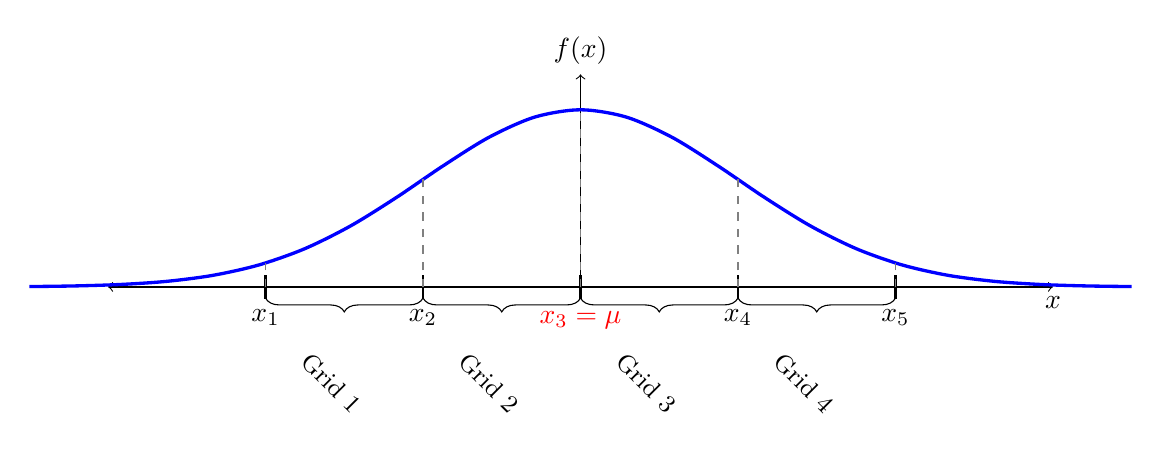
\begin{tikzpicture}[
    % Set a scale for better visibility
    xscale=2, yscale=1.5
]



% --- Define Parameters ---
\def\mean{0}      % Set mean to 0 for simplicity
\def\stdev{1}     % Standard deviation for the normal curve shape
\def\gridstep{1} % Distance between grid points (e.g., 1 * stdev)

% --- Define Grid Points ---
% 5 points are needed to create 4 segments (2 on each side of the mean)
\pgfmathsetmacro{\xone}{\mean - 2*\gridstep}
\pgfmathsetmacro{\xtwo}{\mean - 1*\gridstep}
\pgfmathsetmacro{\xthree}{\mean}
\pgfmathsetmacro{\xfour}{\mean + 1*\gridstep}
\pgfmathsetmacro{\xfive}{\mean + 2*\gridstep}

% --- Draw Axes ---
% X-axis
\draw [<->] (\mean - 3.0*\gridstep, 0) -- (\mean + 3.0*\gridstep, 0) node[below] {$x$};
% Y-axis (optional, for context)
\draw [->] (0, 0) -- (0, 1.8) node[above] {$f(x)$};

% --- Draw Normal Distribution Curve ---
% We use exp(-x^2 / (2*stdev^2)). 
% The '1.5' is a scaling factor for the height to make it look good.
\draw[blue, very thick, domain=\mean - 3.5*\stdev:\mean + 3.5*\stdev, smooth] 
    plot (\x, {1.5 * exp(-(\x - \mean)^2 / (2 * \stdev^2))});
    
% --- Mark Grid Points on X-Axis ---
% Draw tick marks and labels for the 5 grid points
\draw[thick] (\xone, 0.1) -- (\xone, -0.1) node[below] {$x_1$};
\draw[thick] (\xtwo, 0.1) -- (\xtwo, -0.1) node[below] {$x_2$};
\draw[thick] (\xthree, 0.1) -- (\xthree, -0.1) node[below, yshift=-1pt] {\textcolor{red}{$x_3=\mu$}};
\draw[thick] (\xfour, 0.1) -- (\xfour, -0.1) node[below] {$x_4$};
\draw[thick] (\xfive, 0.1) -- (\xfive, -0.1) node[below] {$x_5$};

% --- Show Discretization ---
% Draw dashed lines from grid points up to the curve
\foreach \xpos in {\xone, \xtwo, \xthree, \xfour, \xfive}
{
    \pgfmathsetmacro{\yval}{1.5 * exp(-(\xpos - \mean)^2 / (2 * \stdev^2))}
    \draw[gray, dashed] (\xpos, 0) -- (\xpos, \yval);
}

% --- Label the Segments ---
% Use braces to clearly show the 4 segments
% Segment 1 (Left)
\draw[decorate, decoration={brace, amplitude=5pt, raise=4pt,mirror}] (\xone, 0) -- (\xtwo, 0) 
    node[midway, below, yshift=-30pt,rotate=-45] {\small Grid 1};
% Segment 2 (Left)
\draw[decorate, decoration={brace, amplitude=5pt, raise=4pt,mirror}] (\xtwo, 0) -- (\xthree, 0) 
    node[midway, below, yshift=-30pt,rotate=-45] {\small Grid 2};
% Segment 3 (Right)
\draw[decorate, decoration={brace, amplitude=5pt, raise=4pt,mirror}] (\xthree, 0) -- (\xfour, 0) 
    node[midway, below, yshift=-30pt,rotate=-45] {\small Grid 3};
% Segment 4 (Right)
\draw[decorate, decoration={brace, amplitude=5pt, raise=4pt,mirror}] (\xfour, 0) -- (\xfive, 0) 
    node[midway, below, yshift=-30pt,rotate=-45] {\small Grid 4};
    
\end{tikzpicture}
\caption{Tauchen discretisation.}
\label{fig:a2_tauchen}
\end{figure}

\colorbox{Cerulean!25}{\textbf{\textit{\underline{Step 2}}} Tauchen discretisation: } \texttt{fnTauchenLogNormal} allows for conducting a quick Tauchen discretisation under the assumption that $z$ follows $\log \mathcal{N}\left(0, \sigma_z \right)$, as visualised on Figure \ref{fig:a2_tauchen}.
\\

\colorbox{Cerulean!25}{\textbf{\textit{\underline{Step 3}}} Probabilistic labour supply decision: } 
Given the presence of the Gumbel \say{shock} in the participation decision, the conditional decisions to participate, $d_v$ and $d_s$, are governed by the following binary probabilities:
\begin{subequations}
    \begin{align}
        & \mathbb{P} \left( d_v = 1 \right) = \frac{\exp \left( \frac{W}{\zeta} \right)}{\exp \left( \frac{W}{\zeta} \right)+\exp \left( \frac{N}{\zeta} \right)}
    \end{align}
    and 
    \begin{align}
        & \mathbb{P} \left( d_s = 1 \right) = \frac{\exp \left( \frac{\varphi W + (1-\varphi)N - \phi}{\zeta} \right)}{\exp \left( \frac{\varphi W + (1-\varphi)N - \phi}{\zeta} \right)+\exp \left( \frac{N}{\zeta} \right)}.
    \end{align}
\end{subequations}




%------------------------------------------------------------------------
%Useful Snippets.
%------------------------------------------------------------------------
%\section{Own Snippets (Comment Out)}
%\vspace{3mm}
%
%% 1. Code Listing. 
%\begin{lstlisting}[frame=single,language=Matlab]
%	An example of Matlab code listing.      
%\end{lstlisting}
%
%% 2. Highlighting.
%\colorbox{maroon!10}{An example of highlighted text.}	
%
%%3. Two Figures Next to Each Other.
%\begin{figure}[hbt]
%\centering
%\begin{subfigure}{.5\textwidth}
%  \centering
%  \includegraphics[width=\linewidth]{}
%  \caption{A}
%\end{subfigure}%
%\begin{subfigure}{.5\textwidth}
%  \centering
%  \includegraphics[width=\linewidth]{}
%  \caption{B}
%\end{subfigure}
%\caption{Two Figures Next to Each Other}
%\label{two_figures}
%\end{figure}	

%------------------------------------------------------------------------
%Bibliography.
%------------------------------------------------------------------------

%\newpage
%
%\bibliographystyle{apalike}
%\bibliography{bibliography}


\printbibliography
\end{document}